\chapter{Dataset \& Experimental Setup}
\label{chap:dataset_experimental_setup}

In the following, we will outline the experimental setup for the experiments we ran.
This includes not only allocation, preprocessing and pair selection of each dataset, but also a description and motivation of the experiments carried out.


\section{Dataset}
\label{sec:dataset}

Since our method extends the original \impAppr{} proposed by \citet{koppel_determining_2014}, we first obtained the datasets used in their study to validate our implementation and reproduce their results. 
The original experiments were conducted on the \dataBlog{} and \dataStudent{} datasets, which are described in detail in \autoref{subsec:original_data}. 
In addition to these, we incorporated two supplementary datasets, \dataPan{} and \dataGutenberg{}, presented in \autoref{subsec:additional_data}. 
Following the general description of all datasets, we outline our preprocessing pipeline in \autoref{subsec:dataset_preprocessing} and conclude with the text-pair selection procedure in \autoref{subsec:dataset_text_pair_selection}.


\subsection{Original Data}
\label{subsec:original_data}

% Blog
The \dataBlog{} corpus~\citep{blog_dataset_2006} consists of blog posts collected from \textit{blogger.com} on or before August 2004, with each blog authored by a single user.
According to the Kaggle repository~\footnote{\href{https://www.kaggle.com/datasets/rtatman/blog-authorship-corpus?resource=download}{Kaggle dataset \texttt{rtatman/blog-authorship-corpus}} (26.07.2025)}, the dataset contains \num{681288} posts from \num{19320} bloggers, averaging approximately 35 posts and \num{7250} words per author.
Users are grouped into three age categories: 13-17, 23-27, and 33-47.
Each record includes the following metadata: \texttt{id}, \texttt{gender}, \texttt{age}, \texttt{topic}, 
\texttt{sign} (referring to the author's astrological/zodiac sign), \texttt{date}, and \texttt{text}.

% student essays
The \dataStudent{} dataset is not publicly available due to the presence of sensitive student information. 
We gratefully acknowledge J. W. Pennebaker for granting access to the original data used by \citet{koppel_determining_2014} in their study. 
The dataset comprises \num{7052} student essays written for five assignments by a cohort of 950 university students in 2006~\citep{koppel_determining_2014}.

The assignments include (1) a stream-of-consciousness task, (2) a reflections on childhood, (3) a self-assessment of personality, (4) a thematic apperception test, and (5) four examples of four different theories.
An inconsistency in the file naming convention is notable: 
Most files are named solely by the author ID, whereas those from the first assignment follow the format \texttt{2006\_authorID}.
Following \citet{koppel_determining_2014}, our \impAppr{} experiments employ only the first four assignments. 
Consistent with \citet{koppel_determining_2014}, disputed–candidate pairs in our setup are drawn from different assignments, irrespective of their class label (\texttt{same-author} or \texttt{different-author}).
In contrast to the original \impAppr{}, which truncated each essay to the first 500 words, we crop texts to the minimum length of the text pair.

Due to privacy restrictions, researchers seeking access to the \dataStudent{} dataset should contact J. W. Pennebaker, the official data custodian. 
For establishing a baseline in our \imp{} experiments, we use both the \dataBlog{} and \dataStudent{} datasets.


\subsection{Additional Data}
\label{subsec:additional_data}
To broaden the evaluation scope of the \impAppr{}, we incorporated additional datasets selected according to two criteria:
(1) control over confounding factors such as genre and topic, and 
(2) verified, undisputed authorship.
Both the \dataPan{} and \dataGutenberg{} datasets satisfy these conditions.

% PAN20: Fanfiction
The \dataPan{} corpus~\citep{bischoff_importance_2020} comprises fanfiction texts sourced from \textit{fanfiction.net}.
Each text belongs exclusively to one fandom (i.e. thematic category), with no crossovers between fandoms.
According to \href{https://pan.webis.de/clef20/pan20-web/author-identification.html}{the official \ac{pan} website}, 
train and test set originate from two different fanfictions and approximate the (long-tail) distribution of the fandoms in the original dataset.
Dataset features include \texttt{id}, \texttt{fandoms}, and \texttt{pair}, where the latter contains the paired texts.
An additional \texttt{jsonl} file provides the ground truth for each pair, specifying \texttt{id}, \texttt{same} (authorship label), and \texttt{authors}.

% Gutenberg
The \dataGutenberg{} dataset~\footnote{\href{https://www.gutenberg.org/}{Project Gutenberg} (26.07.2025)} contains a curated selection of literary works from Project Gutenberg, a digital library dedicated primarily to older works whose U.S. copyrights have expired.
As of this writing, the collection contains over \num{75000} digitized and proofread e-books contributed by volunteers.
For our experiments, we selected 19 works authored by 7 writers from the 16th to 19th centuries, covering genres such as drama, fiction, and poetry.
Metadata for these works was manually extracted from the Project Gutenberg website and Wikipedia.


\subsection{Dataset Preprocessing}
\label{subsec:dataset_preprocessing}

To control confounding factors that influence authorial style, we preprocess each dataset twice:
(1) Prior to generating arrow dataset file and (2) before using the \impAppr{}.
This two-stage approach addresses both experimental scenarios, where all material is prepared in advance, and inference scenarios in which the \impAppr{} model is applied directly to texts.
The preprocessing process was designed to meet the following requirements:
\begin{itemize}
    \item Removal of all formatting and layout information to produce plain text.
    \item Cropping texts to match the length of the shorter text in each pair.
\end{itemize}
It is important to note that text-length adjustment is performed exclusively within the \impAppr{} implementation and is not applied to the Arrow dataset itself.
For a controlled evaluation environment in our \impAppr{}, we opted to work with relatively small, curated datasets rather than scaling to larger collections.  
The effect of individual preprocessing steps on vocabulary size was analysed, with results presented in \autoref{fig:preprocesing_impact_vocab_size}.
In line with \citep{koppel_determining_2014}, the vocabulary consists of space-free character 4-grams.
Removing formatting and layout information includes removing HTML artefacts, play artefacts, newlines, 
converting UTF-8 to ASCII, and stripping leading and trailing whitespace.
Since both \dataBlog{} and \dataPan{} originate from the Internet, we applied HTML-specific preprocessing steps, which had minimal impact on their respective vocabularies.
Upon inspection of the \dataGutenberg{}, we found that certain patterns reappear due to the \textit{play} genre. 
Notably, since we do not consider actor instructions (e.g., character cues) or structural elements (e.g., chapter headings) as part of authorial style, these patterns were removed using regular expressions.
We opted to forgo lowercasing the texts, as our preliminary analysis indicated that lowercasing had no meaningful effect on any dataset while potentially discarding deliberate authorial capitalization choices.

\begin{figure}[htbp]
    \centering
    \includesvg[width=\textwidth]{images/dataset/impact_preprocessing_steps.svg}
    \caption{Effect of preprocessing steps on vocabulary size (space-free character 4-grams).}
    \label{fig:preprocesing_impact_vocab_size}
\end{figure}

\subsection{Selection of Text Pairs}
\label{subsec:dataset_text_pair_selection}

We had to select pairs of texts for the \dataBlog{}, \dataStudent{} and the \dataGutenberg{} dataset.
Eligible texts have a minimum length of \num{700} words for all datasets.
% We select a lower limit of \num{500} words for the \dataStudent{} dataset, 
% since the longest essay only contains \num{1136} words.
We decided to keep the existing pairs in the \dataPan{} arrow dataset for better comparability.
All datasets consist of same- and different-author pairs. 
As mentioned before, we aimed to control confounders when selecting pairs.
Find descriptive statistics for the preprocessed datasets in Table~\ref{tab:data_stats}.

% minimum length necessesary for AV/ AA
When selecting the minimum length of texts, we consulted related research in the field of \ac{av} and \ac{aa}.
\citet{bevendorff_generalizing_2019} use texts chunks of at least 700 words for their unmasking approach, 
where \citet{koppel_authorship_2004} set the minimum length to 500 words.
Recent work~\citep{llm_detection_av_2025} identifies a minimum length of \num{2500}-\num{4000} characters 
sufficient for effective \ac{llm} detection (framed as \ac{av} or \ac{aa}).
Therefore, they opted for a minimum length of \num{3000} characters for their datasets.

Their statistical properties are summarized in \autoref{tab:data_stats}.

% \begin{table}[h]
\begin{sidewaystable}
\centering\small
\caption{Statistics of preprocessed datasets \dataPan{}, \dataBlog{}, \dataGutenberg{}, and \dataStudent{}.}
\label{tab:data_stats}
\resizebox{\textwidth}{!}{%
\begin{tabular}{@{}lrrrrrrrrr@{}}   % numbers should be right aligned, text left aligned
\toprule
dataset & num\_pairs & num\_authors & num\_same\_pairs & num\_different\_pairs & avg\_text\_len & max\_text\_len\_words & std\_text\_len\_words & median\_text\_len\_words \\
\midrule
pan20           & 66905 & 52771 & 35616 & 31289 & 21418.76 (3914.76)   & 55413 & 512.19 & 3889 \\
blog            & 11565 & 5997  & 6204 & 5361  & 6249.94 (1154.25)     & 115365 & 1493.97 & 913 \\
gutenberg       & 12    & 7     & 6     & 6     & 437870.75 (78698.79) & 297704 & 68329.91 & 60282 \\
student\_essays & 224  & 222   & 112   & 112  & 4459.32 (865.90)     & 1634 & 157.41 & 815  \\
\bottomrule
\end{tabular}%
}
% \end{table}
\end{sidewaystable}

For the \dataBlog{} dataset, 
two texts of a pair are selected such that they share the same topic, year, gender and age, where the last to reference the text's author.
Train (80\%) and test split (20\%) have different topics.

For the \dataStudent{} dataset,
tasks are either in the train (70\%) or test (30\%) set.
The test set is bigger, since an author typically only writes one essay per task and if only one task is selected for the test set we can not create any same author pairs.
The pairs are selected such that their authors share the same sex, ethnicity, and political orientation.
Additionally, for different author pairs, the texts are selected such that they share the same task.

For the \dataGutenberg{} dataset,
we selected pairs of texts that share the same genre and century.
Authors can either be in the train (80\%) or test (20\%) set.

Irrespective of the information used to select pairs, the final dataset contains only the columns \texttt{authors}, \texttt{pair}, and \texttt{same}.
The \texttt{pair} column contains the texts of the pair as a list of strings,
the \texttt{authors} column contains the authors of the texts as a list of strings,
and the \texttt{same} column indicates whether the texts are from the same author (\texttt{True}) or from different authors (\texttt{False}).


\section{Experimental Setup}
\label{sec:experimental_setup}

\subsection{Reproducing \citet{koppel_determining_2014}' Experiments}

\subsection{Exp.\ 3: Paraphrasing Chunks}
\label{subsec:paraphrasing_chunks_setup}

We designed this experiment to evaluate whether chunk-to-chunk paraphrases exhibit better control than text-to-text paraphrases, since chunks contain fewer topic changes than whole texts in theory.
We use one text from the \dataBlog{}, \dataGutenberg{}, and the \dataStudent{} dataset, respectively.


\begin{figure}[htbp]
  \centering
  \includesvg[width=\linewidth]{images/paraphrasing/experiments/chunks/setup/chunk_api_calls.svg}
  \caption[Paraphrase configuration hyperparameters]{Breakdown of individual hyperparameters in the paraphrase configuration.
  We use one document per dataset, chunked into one to five sections and paraphrased with all nine paraphrasers in two variance inducing settings (i.e.\ prompt for one-step, temperature for two-step).
  This amounts to a total of 936 API calls. 
  }
  \label{fig:chunks_api_calls}
\end{figure}


First, texts are chunked preserving sentences.
Chunks are filled with sentences in sentence order such that each chunk roughly contains the same number of words.
Second, paraphrase configurations are defined.
Each one-step paraphraser is paired with two prompts (i.e.\ \texttt{prompt0} and \texttt{prompt1} from \Cref{subsec:one_step_paraphrasing_prompts}), while each two-step paraphraser is paired with two temperatures (i.e.\ 0 and 1).
Third, each chunk is paraphrased with all configurations.
These steps account for a minimum of 936 API calls for paraphrasing.
Each component of the configuration is displayed in \Cref{fig:chunks_api_calls}.
Finally, for each paraphrase, we compute \ac{bleu}, \ac{rouge}-1, \ac{rouge}-2, \ac{rouge}-L, \ac{rouge}-Lsum, \ac{meteor}, \ac{bert}\-Score Precision, \ac{bert}\-Score Recall, \ac{bert}\-Score F1, \ac{sbert} \ac{wms}, and \ac{sbert} cosine similarity.
Final scores per metric for each text-configuration pair are computed by averaging the scores of its constituent text chunks.
The adequate formula is given in \Cref{eq:avg_chunks} and an example is illustrated in \Cref{fig:mean-bleu}.

\begin{equation}
    score(t) = \frac{1}{\#\text{ chunks}}\sum_{i=1}^{\#\text{ chunks}}score(c_i)\text{, for chunk }c_i \in \text{text }t
\label{eq:avg_chunks}
\end{equation}

\begin{figure}[ht]
  \centering
\resizebox{0.9\textwidth}{!}{%
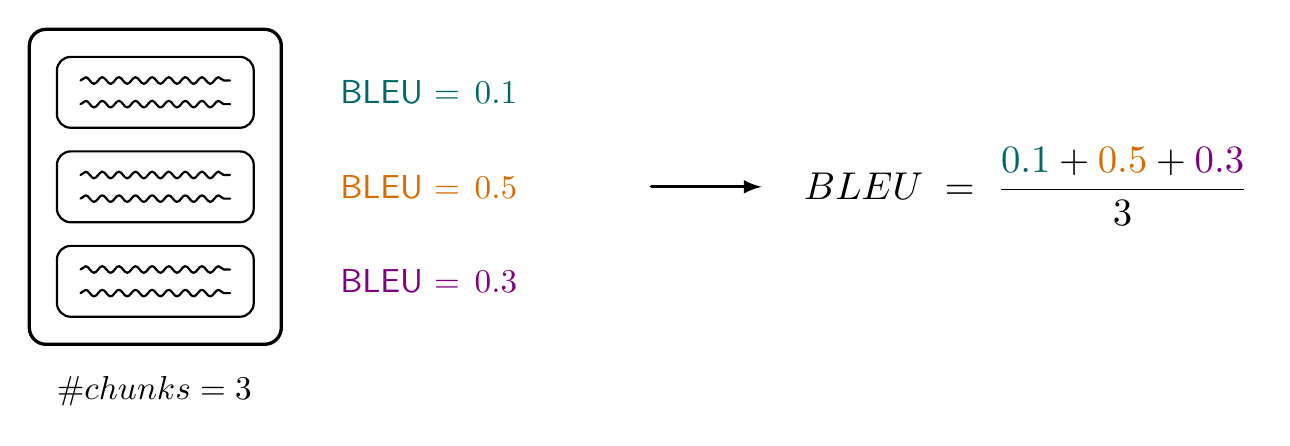
\begin{tikzpicture}[line join=round,line cap=round, >=latex, font=\sffamily]

% --- Left black container with three chunks ---
\draw[black, very thick, rounded corners=6pt]
  (-0.2,3.6) rectangle (3.0,-0.4);

% three inner rounded rectangles
\foreach \y in {2.8,1.6,0.4}{
  \draw[black, thick, rounded corners=5pt] (0.15,\y+0.45) rectangle (2.65,\y-0.45);
  % squiggle inside
  \draw[black, thick, decorate, decoration={snake,amplitude=1.2pt,segment length=6pt}]
    (0.45,\y-0.15) -- (2.35,\y-0.15);
  \draw[black, thick, decorate, decoration={snake,amplitude=1.2pt,segment length=6pt}]
  (0.45,\y+0.15) -- (2.35,\y+0.15);
}

% --- Colored BLEU labels next to each chunk ---
\node[anchor=west, text=teal!80!black, scale=1.2]  at (3.6,2.8) {BLEU $=\,0.1$};
\node[anchor=west, text=orange!85!black, scale=1.2] at (3.6,1.6) {BLEU $=\,0.5$};
\node[anchor=west, text=violet, scale=1.2]         at (3.6,0.4) {BLEU $=\,0.3$};

% --- n_chunks = 3 (black) ---
\node[anchor=west, text=black, scale=1.2] at (0.0,-1.0) {$\#\text{ chunks}=3$};

% --- Arrow to the right and mean BLEU expression ---
\draw[black, very thick, ->, >=latex] (7.7,1.6) -- (9.1,1.6);

\node[anchor=west, text=black, scale=1.4] at (9.3,1.6)
  {$\varnothing\ \text{BLEU} \;=\; \displaystyle
   \frac{\textcolor{teal!80!black}{0.1}+\textcolor{orange!85!black}{0.5}+\textcolor{violet}{0.3}}{3}$};

\end{tikzpicture}
}
  \caption[Computation of the mean \ac{bleu} score over chunks]{Computation of the mean \ac{bleu} score over three text chunks of a text.}
  \label{fig:mean-bleu}
\end{figure}


\subsection{Comparison of different Paraphrasers with Reference Text}

\subsection{Impact of syntactic similarity on \imp{} Detector scores}
\label{sec:syn_sim_impact_}

\subsection{Naive Paraphrasers and \acp{fp}}

\subsection{Comparing \citet{koppel_determining_2014}'s to \ac{llm}-based \imps{}}

\subsection{Comparing Different \ac{av} Models}





